\documentclass{beamer}
\usetheme{Boadilla}
\usepackage{hyperref}
\usepackage{graphicx}
\usepackage{fancyvrb}
\usepackage{multicol}
\usepackage{subfig}
\usepackage[
    backend=biber, 
    natbib=true,
    style=numeric,
    sorting=none,
    style=verbose-ibid,
]{biblatex}
\addbibresource{citations.bib}
\usepackage{pgfpages}
\usepackage{xcolor}
\definecolor{ao(english)}{rgb}{0.0, 0.5, 0.0}
\definecolor{burgundy}{rgb}{0.5, 0.0, 0.13}
%\setbeameroption{show notes}
\setbeameroption{show notes on second screen=right}
%\setbeameroption{hide notes}

\title{Gabor's 1946 Theory of Communication}
\author{Sevag Hanssian}
\institute{MUMT 622, Winter 2021}
\setbeamertemplate{navigation symbols}{}

\begin{document}

\begin{frame}
\maketitle
\end{frame}

\begin{frame}
	\frametitle{Time-frequency resolution in the STFT}
	\begin{figure}
		\centering
		\subfloat[Good time resolution, poor frequency resolution]{{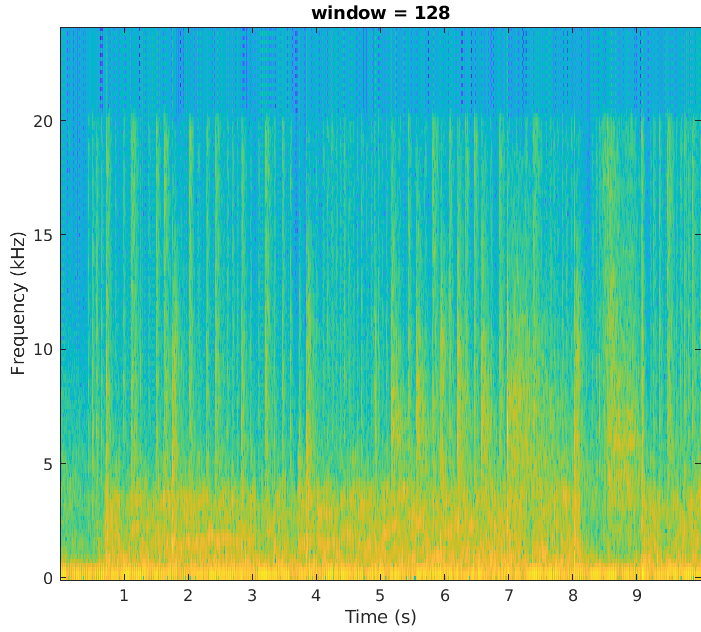
\includegraphics[width=6cm]{./stft_small.png} }}
		\subfloat[Good frequency resolution, poor time resolution]{{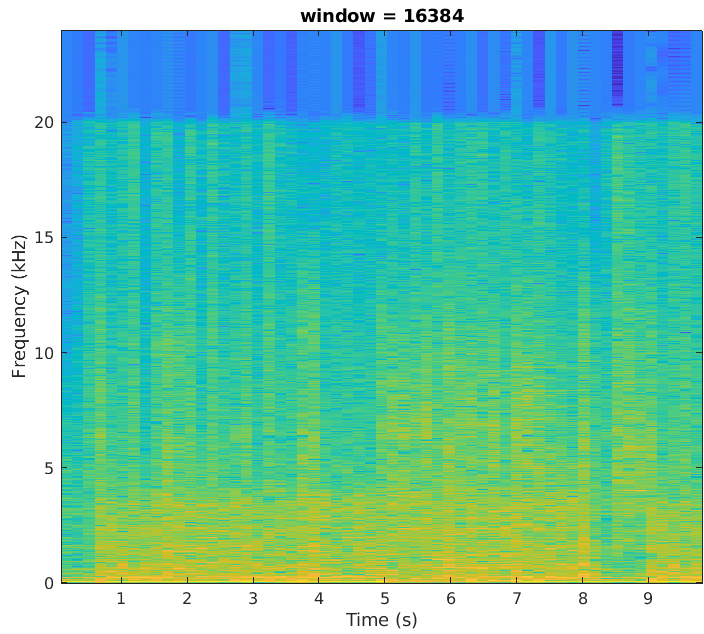
\includegraphics[width=6cm]{./stft_big.png} }}
		\caption{STFT, small vs. big window}
	\end{figure}
\end{frame}

\begin{frame}
	\frametitle{Time-frequency resolution in the STFT}
	\begin{figure}
		\centering
		\subfloat[Good time resolution, poor frequency resolution]{{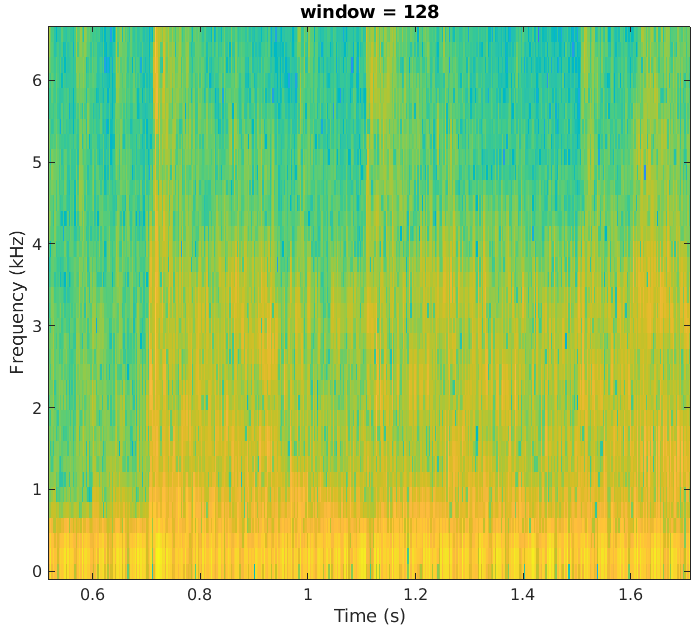
\includegraphics[width=6cm]{./stft_small_zoomed.png} }}
		\subfloat[Good frequency resolution, poor time resolution]{{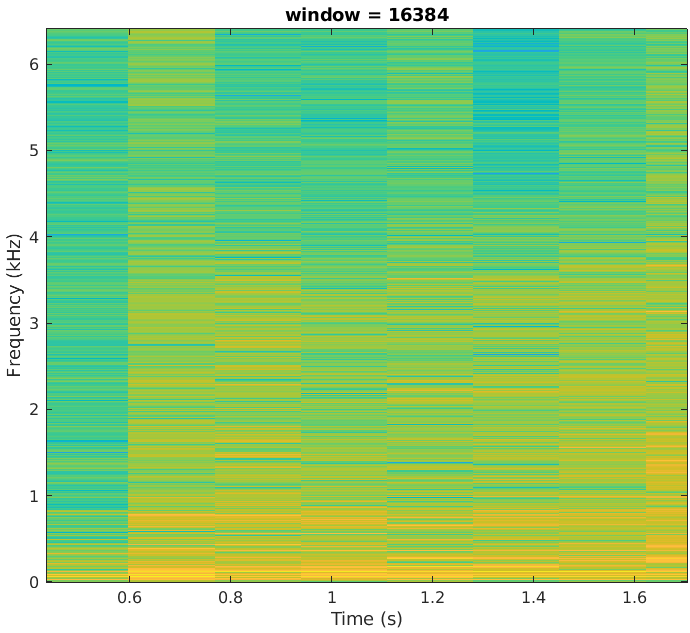
\includegraphics[width=6cm]{./stft_big_zoomed.png} }}
		\caption{STFT, small vs. big window}
	\end{figure}
\end{frame}

\begin{frame}
	\frametitle{Signals in time and frequency}
	\begin{figure}
		\centering
		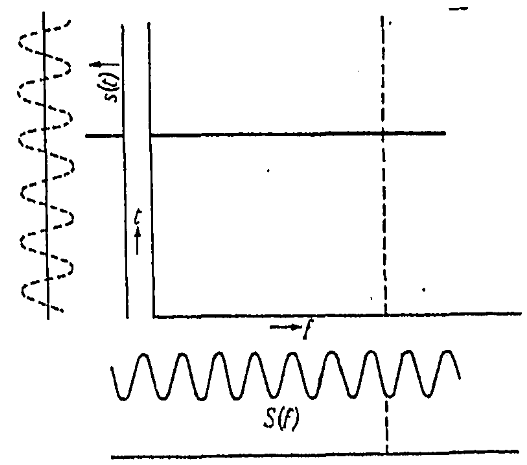
\includegraphics[width=6cm]{./gabor1.png}
		\caption{Unit impulse (delta function) and infinite sine wave in time/frequency diagram\footfullcite{gabor1946}}
	\end{figure}
\end{frame}

\end{document}
